\documentclass[tikz, border=10pt]{standalone}
\usepackage{amsmath}
\usetikzlibrary{positioning, arrows.meta, backgrounds, calc, shapes.geometric}

% ==========================================
% 高级柔和配色 (适合正式论文)
% ==========================================
\definecolor{b1fill}{RGB}{235, 245, 255}
\definecolor{b1draw}{RGB}{21, 101, 192}
\definecolor{b2fill}{RGB}{249, 251, 235}
\definecolor{b2draw}{RGB}{130, 119, 23}
\definecolor{b3fill}{RGB}{255, 240, 240}
\definecolor{b3draw}{RGB}{192, 57, 43}

\definecolor{opfill}{RGB}{245, 247, 250}
\definecolor{opdraw}{RGB}{84, 110, 122}
\definecolor{rezero}{RGB}{255, 243, 224}

\begin{document}
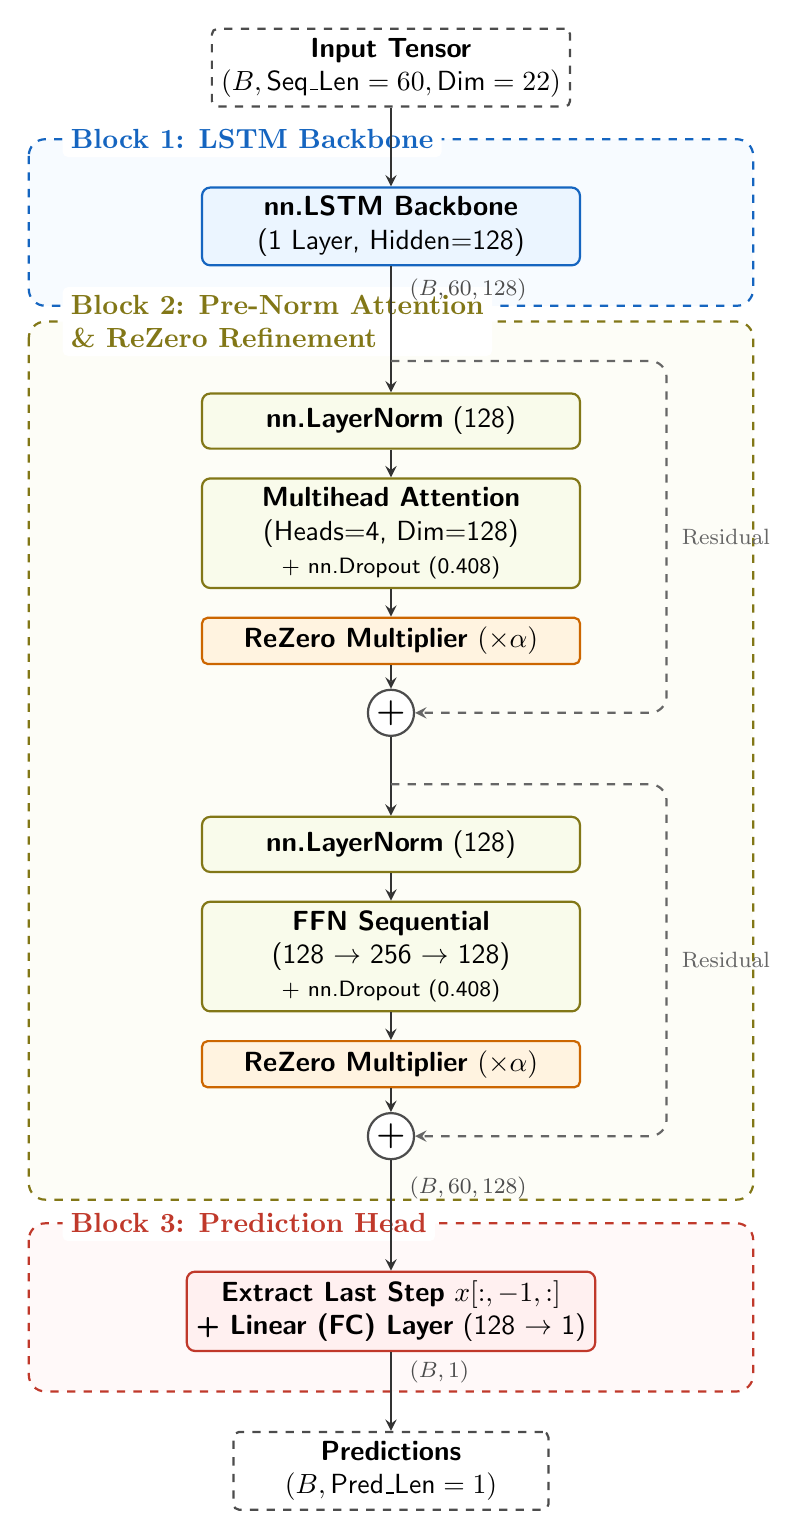
\begin{tikzpicture}[
    >=stealth,
    font=\sffamily,
    tensor/.style={draw=black!70, dashed, fill=white, minimum width=4cm, minimum height=0.6cm, align=center, thick, rounded corners=2pt},
    layer/.style={draw=#1draw, fill=#1fill, rounded corners=3pt, minimum width=4.8cm, minimum height=0.7cm, align=center, thick},
    rezero_op/.style={draw=orange!80!black, fill=rezero, rounded corners=2pt, minimum width=4.8cm, minimum height=0.5cm, align=center, thick},
    add/.style={draw=black!70, fill=white, circle, inner sep=1pt, minimum size=0.5cm, font=\large\bfseries, thick},
    arrow/.style={->, thick, draw=black!80, rounded corners=4pt},
    resarrow/.style={->, thick, dashed, draw=black!60, rounded corners=6pt},
    groupbox/.style={draw=#1draw, thick, dashed, rounded corners=6pt, fill=#1fill!40}
]

% ==========================================
% 1. 模型主体节点绘制
% ==========================================
\node[tensor] (input) {\textbf{Input Tensor}\\ $(B, \text{Seq\_Len}=60, \text{Dim}=22)$};

\node[layer=b1, below=1.0cm of input] (lstm) {\textbf{nn.LSTM Backbone}\\(1 Layer, Hidden=128)};

\coordinate[below=1.2cm of lstm] (split1);

\node[layer=b2, below=0.4cm of split1] (norm1) {\textbf{nn.LayerNorm} (128)};
\node[layer=b2, below=0.35cm of norm1] (mha) {\textbf{Multihead Attention}\\(Heads=4, Dim=128)\\ \footnotesize{+ nn.Dropout (0.408)}};
\node[rezero_op, below=0.35cm of mha] (rezero1) {\textbf{ReZero Multiplier} $(\times \alpha)$};
\node[add, below=0.3cm of rezero1] (add1) {+};

\coordinate[below=0.6cm of add1] (split2);

\node[layer=b2, below=0.4cm of split2] (norm2) {\textbf{nn.LayerNorm} (128)};
\node[layer=b2, below=0.35cm of norm2] (ffn) {\textbf{FFN Sequential}\\(128 $\to$ 256 $\to$ 128)\\ \footnotesize{+ nn.Dropout (0.408)}};
\node[rezero_op, below=0.35cm of ffn] (rezero2) {\textbf{ReZero Multiplier} $(\times \alpha)$};
\node[add, below=0.3cm of rezero2] (add2) {+};

\node[layer=b3, below=1.4cm of add2] (head) {\textbf{Extract Last Step} $x[:, -1, :]$\\ \textbf{+ Linear (FC) Layer} (128 $\to$ 1)};

\node[tensor, below=1.0cm of head] (output) {\textbf{Predictions}\\ $(B, \text{Pred\_Len}=1)$};

% ==========================================
% 2. 绘制背景区域 (保持绝对坐标以杜绝形变)
% ==========================================
\begin{scope}[on background layer]
    \coordinate (B1_top) at ($(lstm.north) + (0, 0.6cm)$);
    \coordinate (B1_bot) at ($(lstm.south) + (0, -0.5cm)$);
    \coordinate (B1_NW) at ($(B1_top) + (-4.6cm, 0)$);
    \coordinate (B1_SE) at ($(B1_bot) + (4.6cm, 0)$);
    \filldraw[groupbox=b1] (B1_NW) rectangle (B1_SE);

    \coordinate (B2_top) at ($(split1) + (0, 0.5cm)$);
    \coordinate (B2_bot) at ($(add2.south) + (0, -0.5cm)$);
    \coordinate (B2_NW) at ($(B2_top) + (-4.6cm, 0)$);
    \coordinate (B2_SE) at ($(B2_bot) + (4.6cm, 0)$);
    \filldraw[groupbox=b2] (B2_NW) rectangle (B2_SE);

    \coordinate (B3_top) at ($(head.north) + (0, 0.6cm)$);
    \coordinate (B3_bot) at ($(head.south) + (0, -0.5cm)$);
    \coordinate (B3_NW) at ($(B3_top) + (-4.6cm, 0)$);
    \coordinate (B3_SE) at ($(B3_bot) + (4.6cm, 0)$);
    \filldraw[groupbox=b3] (B3_NW) rectangle (B3_SE);
\end{scope}

% ==========================================
% 3. 绘制框体标签
% ==========================================
\node[fill=white, font=\bfseries\color{b1draw}, right=12pt, rounded corners=2pt, inner sep=3pt] 
    at (B1_NW) {Block 1: LSTM Backbone};

\node[fill=white, font=\bfseries\color{b2draw}, right=12pt, align=left, rounded corners=2pt, inner sep=3pt] 
    at (B2_NW) {Block 2: Pre-Norm Attention\\\& ReZero Refinement};

\node[fill=white, font=\bfseries\color{b3draw}, right=12pt, rounded corners=2pt, inner sep=3pt] 
    at (B3_NW) {Block 3: Prediction Head};

% ==========================================
% 4. 连线与标注 
% ==========================================
\draw[arrow] (input) -- (lstm);


\draw[arrow] (lstm) -- node[pos=0.25, right=3pt, font=\footnotesize\color{black!70}] {$(B, 60, 128)$} (split1) -- (norm1);

\draw[arrow] (norm1) -- (mha);
\draw[arrow] (mha) -- (rezero1);
\draw[arrow] (rezero1) -- (add1);

\draw[arrow] (add1) -- (split2) -- (norm2);

\draw[arrow] (norm2) -- (ffn);
\draw[arrow] (ffn) -- (rezero2);
\draw[arrow] (rezero2) -- (add2);

\draw[arrow] (add2) -- node[pos=0.25, right=3pt, font=\footnotesize\color{black!70}] {$(B, 60, 128)$} (head);
\draw[arrow] (head) -- node[pos=0.25, right=3pt, font=\footnotesize\color{black!70}] {$(B, 1)$} (output);

% ==========================================
% 5. 残差跳连线
% ==========================================
\draw[resarrow] (split1) -- ++(3.5,0) coordinate (r1) -- (r1 |- add1) -- (add1.east);
\node[right=2pt, font=\footnotesize\color{black!60}] at ($(r1)!0.5!(r1 |- add1)$) {Residual};

\draw[resarrow] (split2) -- ++(3.5,0) coordinate (r2) -- (r2 |- add2) -- (add2.east);
\node[right=2pt, font=\footnotesize\color{black!60}] at ($(r2)!0.5!(r2 |- add2)$) {Residual};

\end{tikzpicture}
\end{document}